\section{Introduction}

\myworries{ Mention somewhere: limit object parametrized by $\sigma_+$ (variance BM), $\frac{\sigma_{-+}+\nu_-}{\mu}$ (parabolic drift BM), and $\frac{\sigma_{-+}+\nu_-}{\mu^2}$ (intensity of sampling ancestral back-edges). For directed ER, these are all $1$. Maybe also worth mentioning: Two main difficulties compared to \cite{goldschmidtScalingLimitCritical2019} 1. lots of dependence vs lots of independence, 2. unlike \cite{goldschmidtScalingLimitCritical2019}, we do not have access to results in the literature on our model, because the configuration model at criticality has not been studied before.}

\subsection{Overview}

Edges in real-world networks are often directed, such as links on the world wide web, follows on Twitter or disease transmission. When analysing networks a natural quantity to consider is are the degrees of nodes in the network.  In this paper we will consider sampling an i.i.d.\ sequence of in- and out-degrees. Conditional on the total in-degree being equal to the total out-degree, we will sample a uniform directed graph (digraph) with the given degree sequence. Results on such graphs provide insight into what additional structure a real-world network has beyond it's degree sequence.

When considering such models, previous work by \citet{cooperSizeLargestStrongly2004} shows that there is a phase transition in the directed connectivity of the graph. Below some threshold, each of the strongly connected components of the graph will contain a negligible proportion of vertices in the graph whereas above the threshold there will exist a unique strongly connected component that occupies a positive proportion of the vertices.  We will study the behaviour of the model at criticality, specifically that there exists a sequence of random weighted directed multigraphs that can be understood as the scaling limit of the strongly connected components when viewed in decreasing order of size.

\subsection{Graph theory}

\begin{figure}
    \centering
    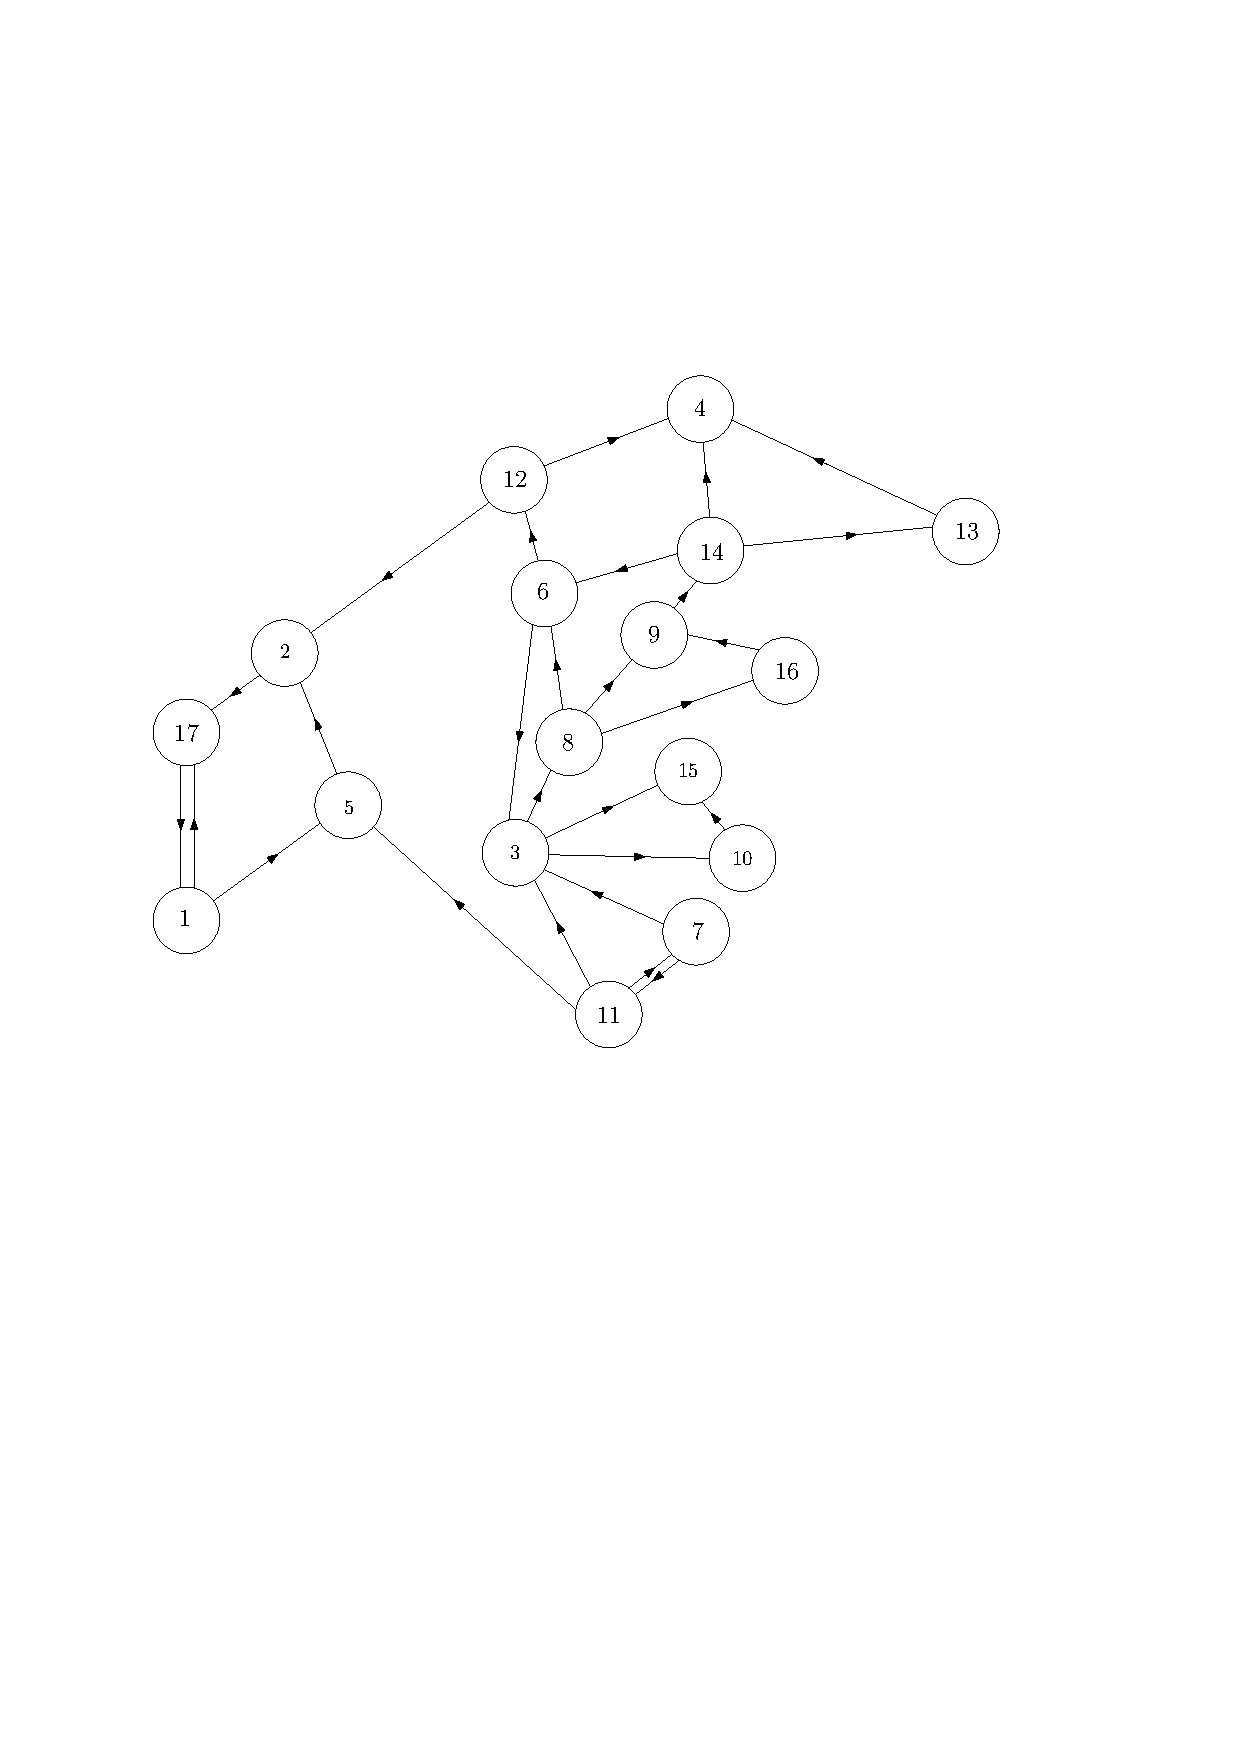
\includegraphics[scale=0.6]{Content/Pictures/biggraph2.pdf}
    \caption{A directed graph on [17]. The strongly connected components have vertex sets $\{1,2,5,17\}$, $\{3,6,8,9,14,16\}$, $\{7,11\}$, $\{4\}$, $\{10\}$, $\{12\}$, $\{13\}$, and $\{15\}$. The figure is created by Goldschmidt and Stephenson \cite{goldschmidtScalingLimitCritical2019}.}
    \label{fig.SCCs}
\end{figure}

There are two notions of connectivity when working with a directed graph - weak and strong connectivity. We will be working with the strong notation. We say a vertex $v$ leads to a vertex $w$ if there exists a directed path from $v$ to $w$ in the graph. We say $v$ is strongly connected to $w$ if $v$ leads to $w$ and $w$ leads to $v$. A graph is strongly connected if any pair of vertices in the graph are strongly connected. The relation is an equivalence relation. The digraphs induced by the equivalence classes of are referred to as the strongly connected components (SCCs).

\subsection{Description of the model}

We consider $n$ vertices, to each of which we assign an in-degree and an out-degree. The degree tuples are independent and identically distributed with law $\nu$. For each $i\in [n]$, let $\mathbf{D}_i=(D^-_i,D^+_i)$ be the in- and out-degree of vertex $i$. In order for a graph with this degree sequence to exist, we require that $\sum_{i=1}^n D^-_i=\sum_{i=1}^n D^+_i$, so we will condition on this event. Conditional on $(\mathbf{D}_1,\dots,\mathbf{D}_n)$, sample a uniform digraph with this degree sequence. Denote resulting random digraph by $\vec{G}_n(\nu)$. We are interested in the limit under scaling of the strongly connected components of $\vec{G}_n(\nu)$ as $n\to \infty$.

We require the degree distribution to satisfy the following properties.

\begin{enumerate}
    \item $\E[(D^- + D^+)^3] < \infty$.
    \item $\E[D^-] = \E[D^+]$.
    \item \emph{lattice condition}
\end{enumerate}

The first condition is required to ensure the steps of a random walk used in the proof has finite variance and thus will convergence (under rescaling) to a Brownian motion.

The second condition and third condition makes sure the event $\{\sum_{i=1}^n D^-_i = \sum_{i=1}^n D^+_i\}$ is well behaved. The second condition ensures this is not a large deviation event and the third condition ensures this event has positive probability for all $n \geq 1$. 

\myworries{go over criticality condition}

We define the following parameters, that will determine the behaviour of the strongly connected components in the limit.
\begin{enumerate}
    \item $\mu:=\E[D^-]=\E[D^+]=\E[D^-D^+]$
    \item $\nu_-:=\frac{\E[(D^-)^2]-\mu}{\mu}$ 
    \item $\sigma_-:=\left(\frac{\mu\E[(D^-)^3]-\E[(D^-)^2]^2}{\mu^2}\right)^{1/2}$ 
    \item $\sigma_+:=\left(\frac{\E[D^-(D^+)^2]-\mu}{\mu}\right)^{1/2}$ 
    \item $\sigma_{-+}:=\frac{\E[(D^-)^2D^+]-\E[(D^-)^2]}{\mu}$ 
\end{enumerate}
% \begin{remark}
% Conditions \ref{cond.beta} and \ref{cond.gamma} ensure that the Central Limit Theorem applies to the fluctuations of the first explored in-degrees around their mean. Condition \ref{cond.critical} ensures that the branching process corresponding to the depth-first exploration (i.e. the exploration of the out-components) is critical. Condition \ref{cond.rho} ensures that this branching process has Brownian scaling. Condition \ref{cond.tau} ensures that the covariance of the in- and out-degrees that are discovered first is finite. Condition \ref{cond.iota} ensures that the strongly connected components are $3$-regular. 
% \end{remark}
\subsection{Topology of convergence}

\begin{figure}[htbp]
    \centering

    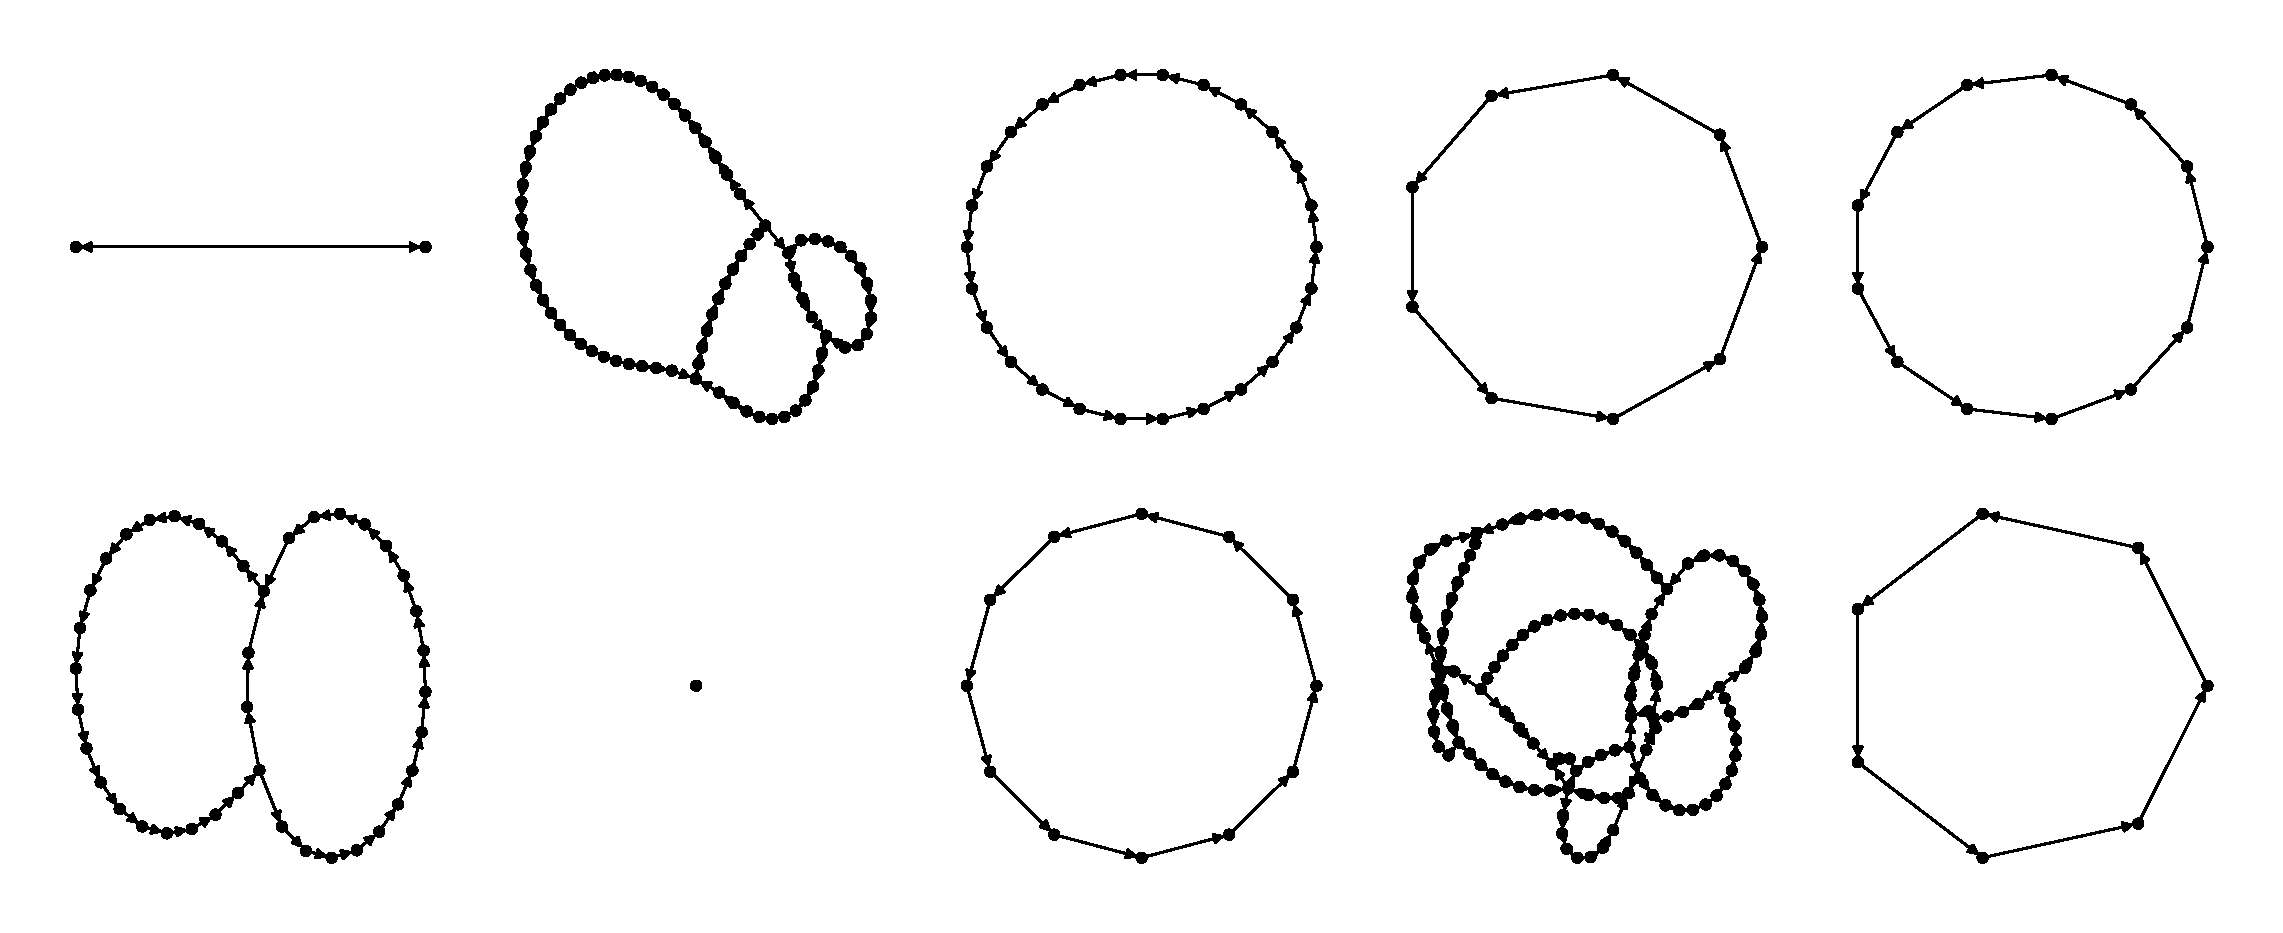
\includegraphics[width=\textwidth]{Content/Pictures/largest_sccs.eps}
    
    \caption{The largest SCC from samples of a directed configuration model with independent $\text{Poisson(1)}$ in- and out-degrees}
    \label{fig:largest-sccs}
\end{figure}

In \cref{fig:largest-sccs} we see the largest SCC from samples of a directed configuration model. As can be seen, while the lengths of paths in the SCC are long, the actual structure of the SCC is often quite simple. Previous work by \citet{goldschmidtScalingLimitCritical2019} shows this is true for the directed Erdős--Renyi model. There it was shown that while the lengths of paths in the SCC will scale like $n^{1/3}$, the actual structure of the SCC will remain finite.

To formalise this idea we will introduce metric directed multigraphs (MDMs). These are simply weighted directed multigraphs, but in our context it is more appropriate to think of the weights as lengths hence the change in naming. Formally a directed multigraph is a tuple $M = (V, E, r)$ where

\subsection{Our results}

Our main result is as follows. Let $C_i(n)$ for $i\geq 1$ be the strongly connected components of $\vec{G}_n(\nu)$, listed in decreasing order of size, breaking ties arbitrarily. We view these strongly connected components as MDMs, by assigning to each edge a length of $1$, and then removing all vertices of degree 2 by merging neighbouring edges and adding up their lengths. Trivial strongly connected components, which consist of an isolated vertex, are considered loops of length $0$. Complete the list with an infinite repeat of $\mathfrak{L}$, the loop of length $0$. Then, the main theorem is as follows.
\begin{theorem}\label{thm.main}
There exists a sequence $\cC=(\cC_i,i\in \N)$ of random strongly connected MDMs such that, for each $i\geq 1$, $\cC_i$ is either $3$-regular or a loop, and such that 
$$\left(n^{-1/3}C_i(n),i\in \N\right)\overset{d}{\to}\left(\cC_i,i\in \N\right)$$
as $n\to \infty$, with respect to the product $d_{\vec{\cG}}$-topology. 
\end{theorem}
The law of the limit object places our model in the universality class of the directed Erd\H{o}s-Rényi model as studied in \cite{goldschmidtScalingLimitCritical2019}. This is the content of the following Corollary.
\begin{corollary}
Consider $\vec{G}_n(\nu)$, with $\nu$ such that $$\sigma_+=1=\frac{\sigma_{-+}+\nu_-}{\mu}=\frac{\sigma_{-+}+\nu_-}{\mu^2}=1.$$ (Note that this condition is satisfied by $\nu(k^-,k^+)=\nu_1(k^-)\nu_2(k^+)$, with $\nu_i$ the law of a $\operatorname{Poisson}(1)$ random variable.)
Let $(C_i(n), i\geq 1)$ be the strongly connected components of $\vec{G}_n(\nu)$, such that by Theorem \ref{thm.main} there exists $\cC=(\cC_i,i\in \N)$ such that 
$$\left(n^{-1/3}C_i(n),i\in \N\right)\overset{d}{\to}\left(\cC_i,i\in \N\right)$$
as $n\to \infty$, with respect to the product $d_{\vec{\cG}}$-topology. Also consider the directed Erd\H{o}s-R\'enyi model on $n$ vertices, in which any directed edge is present independently with probability $1/n$, which we denote by $\vec{G}(n,1/n)$, and let $(C'_i(n), i\geq 1)$ be the strongly connected components of $\vec{G}_n(\nu)$. Then, also
$$\left(n^{-1/3}C'_i(n),i\in \N\right)\overset{d}{\to}\left(\cC_i,i\in \N\right)$$
as $n\to \infty$, with respect to the product $d_{\vec{\cG}}$-topology. 
\end{corollary}
Moreover, Theorem \ref{thm.main} has the following trivial corollaries, which were previously unknown. 
\begin{corollary}
There exists a random sequence $(\ell_i,i\in \N)\in \R_+^\infty$, such that for $(L^n_i,i\in \N)$ the total lengths in the strongly connected components of $\vec{G}_n(\nu)$ ordered by decreasing length (appended with an infinite repeat of $0$), and for $(S^n_i,i\in\N)$ the number of vertices in the the strongly connected components of $\vec{G}_n(\nu)$ ordered by decreasing size (appended with an infinite repeat of $0$),
$$\left(n^{-1/3}L^n_i,n^{-1/3}S^n_i, i\in \N\right)\overset{d}{\to}\left(\ell_i,\ell_i,i\in \N\right)$$
as $n\to \infty$ in the product topology on $(\R^2)^\infty$. 
\end{corollary}
\begin{corollary}
For $v,w\in \vec{G}_n(\nu)$ such that $v\to w$, let $d(v,w)$ denote the length of the shortest path from $v$ to $w$, and let $$\operatorname{Diam}\left(\vec{G}_n(\nu)\right)=\max\{d(v,w):v\to w\}$$ be the \emph{diameter} of $\vec{G}_n(\nu)$. Then,  $$\operatorname{Diam}\left(\vec{G}_n(\nu)\right)=\Omega(n^{1/3})$$
with high probability.
\end{corollary}


\subsection{Previous work}
The configuration model was introduced by Bollobás \cite{Bollobas1980} to sample a uniformly random graph with a given degree sequence. For a discussion of the configuration model and proofs of standard results, we refer the reader to \cite{hofstadRandomGraphsComplex2017}, Chapter 7.   

Most results on the configuration model are obtained for models with a deterministic degree sequence. The phase transition for undirected setting was shown in \cite{molloyCriticalPointRandom1995}, \cite{Molloy1998}, \cite{Janson2009}. The law of component sizes at criticality and in the critical window were obtained by Riordan  under the assumption that the degrees are bounded \cite{Riordan2012}. Dhara, van der Hofstad, van Leeuwaarden and Sen showed convergence of the size and surplus edges in the critical window in the finite 3rd moment setting \cite{Dhara2017} and in the heavy-tailed regime \cite{Dhara2020}.  Bhamadi, Dhara, van der Hofstad and Sen obtained metric space convergence in the critical window in \cite{Bhamidi2020}, a result that the authors later improved to a stronger topology in \cite{Bhamidi2020Glmb}. 

Configuration models with a random degree sequence are considered in \cite{josephComponentSizesCritical2014}, \cite{conchon--kerjanStableGraphMetric2020}, and \cite{Donderwinkel2021heightprocess}. Joseph showed convergence of the component sizes and surpluses of the large components under rescaling at criticality, both for degree distributions with finite third moments and for the heavy-tailed regime \cite{josephComponentSizesCritical2014}. Conchon-Kerjan and Goldschmidt show Gromov-Hausdorff-Prokhorov convergence at criticality in these two regimes \cite{conchon--kerjanStableGraphMetric2020}. The results in \cite{conchon--kerjanStableGraphMetric2020} in the heavy-tailed regime are extended to the critical window by Donderwinkel \cite{Donderwinkel2021heightprocess}. Our techniques are closely related to the techniques introduced in \cite{conchon--kerjanStableGraphMetric2020}. 

Some results have been obtained for other directed graph models. In \cite{caoConnectivityGeneralClass2019}, a class of inhomogeneous directed graphs is considered. Their results include a phase transition for the existence of a giant strongly connected component. This is a generalisation of \cite{Bloznelis2012}, in which a smaller class of inhomogeneous directed graphs is considered. In \cite{Samorodnitsky2016}, the tails of the degree distribution in the directed preferential attachment model are studied. Goldschmidt and Stephenson studied the directed Erd\H{o}s-R\'enyi model, and were the first to obtain metric space convergence of the strongly connected components of a directed graph \cite{goldschmidtScalingLimitCritical2019}. Our methods build on their techniques.

The directed configuration model was first considered by Cooper and Frieze \cite{cooperSizeLargestStrongly2004}. They consider a deterministic degree sequence under a number of conditions, and show that for $\theta$ the expected in-degree of a uniformly chosen vertex, and $\rho$ the expected product of in-degree and out-degree of a uniformly chosen vertex, a phase transition for the strongly connected components occurs at $d=\theta/\rho=1$. They show that for $d<1$, with high probability, all strongly connected components contain $O(\Delta\log(n))$ vertices, for $\Delta$ the maximal degree. On the other hand, for $d>1$, there is a unique strongly connected components that contains a positive proportion of the vertices and also $O(n)$ edges. Their conditions are restrictive, and include finite second moments of both the in- and out-degree of a uniformly chosen vertex, and a bound of size $n^{1/12}/\log(n)$ on the largest degree. Their proofs are based on an algorithm to explore the directed graph. The condition on the largest degree was later relaxed to $O(n^{1/4})$ by Graf \cite{Graf2016}.\\

Recently, Cai and Perarnau have obtained a number of results on the directed configuration model with deterministic degrees. In \cite{caiDiameterDirectedConfiguration2020}, they show, under first and second moment conditions of the degree of a uniformly picked vertex, for $d\neq 1$ (i.e. not at criticality), that the diameter of the model on $n$ vertices, rescaled by $\log(n)$ converges to a constant that they identify. Then, in \cite{caiGiantComponentDirected2020}, they show a law of large numbers for the number of vertices and edges in the largest strongly connected component, under slightly stronger moment conditions, and again not at the critical point. In \cite{cai2021rw}, they study the behaviour of a random walk on a directed configuration model.
 
The emergence of a giant weakly connected component for the directed configuration model with a deterministic degree sequence is discussed in the physics literature by Kryven in \cite{Kryven2016}. He also studies the distribution of the in- and out-components in \cite{Kryven2017}.

The directed configuration model with random in- and out-degrees is only considered by \cite{Chen2012}. The authors consider a model in which the in- and out-degrees are two independent sequences of i.i.d.\ random variables drawn from two probability distributions. They propose an algorithm to sample degree sequences that correspond to a simple graph and show the limiting distribution of the degrees generated by this algorithm. 


\subsection{Proof outline}
The techniques we will use to investigate the graph model are a combination of the techniques introduced by Conchon-Kerjan and Goldschmidt in \cite{conchon--kerjanStableGraphMetric2020} and the strategy of Goldschmidt and Stephenson in \cite{goldschmidtScalingLimitCritical2019}. The former work discusses the scaling limit of an undirected uniform graph with i.i.d.\ degrees at criticality, and the latter discusses the scaling limit of the strongly connected components of a directed Erd\H{o}s-Renyi graph at criticality.\\
To investigate the structure of the strongly connected components of a uniform graph with degree sequence $(\mathbf{D}_1,\dots,\mathbf{D}_n)$, conditional on $\sum_{i=1}^n D^-_i=\sum_{i=1}^n D^+_i$, we will use a version of the configuration model for digraphs that was introduced in \cite{cooperSizeLargestStrongly2004}. The output of the configuration model, conditional on being a simple graph, is a uniform digraph with the given degree sequence. \\
\myworries{Description of exploration written by Zheneng} This is illustrated in Figure \ref{fig.configuration model}. 
\begin{figure}
    \centering
    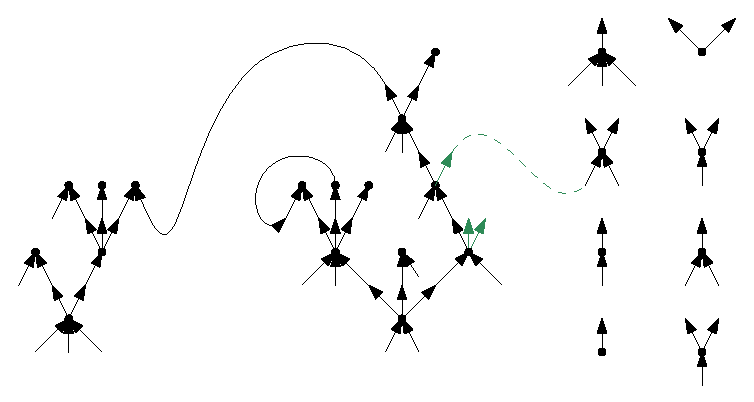
\includegraphics[scale=0.6]{Content/Pictures/configuration_model.eps}
    \caption{The green arrows represent unpaired out-half-edges of vertices that have been visited. One by one, in depth first order, these are paired to a uniform unpaired in-half-edge.}
    \label{fig.configuration model}
\end{figure}\\
The exploration algorithm naturally gives rise to a forest that we will refer to as the \emph{out-forest}, which will play a key role in studying the limit under rescaling of the strongly connected components. An important motivation for studying the out-forest is the fact that the vertex set of any strongly connected component is contained in one of the components of the out-forest. We define the out-forest in such a way that every time step in the exploration corresponds to one vertex in the out-forest. At every time step in the exploration at which we find an unseen vertex, say with out-degree $d^+$, we add a vertex with $d^+$ children to the out-forest. At every time step at which we do not find a new vertex, but instead connect to a previously found vertex, we add a purple leaf to the out-forest. This is illustrated in Figure \ref{fig.configuration modeloutforest}. We refer to the out-forest corresponding to the exploration up to time $k$ as $\hat{F}_n(k)$.\\
A key fact is that the out-forest can be sampled without knowing what the heads of the surplus edges are, because this information does not affect the law of the out-forest. This allows us to build up the randomness of the exploration in the following layers.
\begin{enumerate}
    \item We sample the out-forest $(\hat{F}_n(k),k\geq 1)$. 
    \item We visit the purple vertices in $(\hat{F}_n(k),k\geq 1)$, and for each vertex we sample whether it is the tail of a \emph{candidate}, i.e. whether the corresponding surplus edge is possibly part of a strongly connected component.
    \item We visit the tails of the candidates in depth-first order, and for each of them, sample where the head of the corresponding surplus edge is.
\end{enumerate}

\begin{figure}
    \centering
    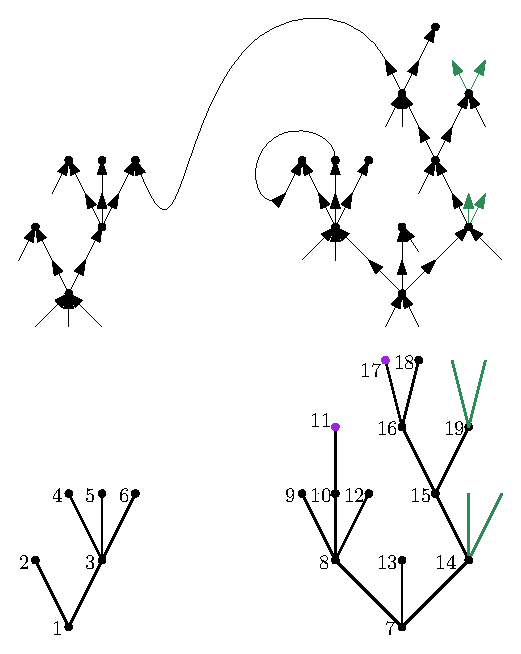
\includegraphics[scale=0.8]{Content/Pictures/configuration_model_out_forest.eps}
    \caption{The out-forest is defined based on the exploration of the digraph. For each surplus edge, we add an extra leaf, which we colour purple. The labels of the vertices correspond to the time step in the exploration at which the vertex is added. The green edges lead to vertices of which the degree and colour have not yet been sampled.}
    \label{fig.configuration modeloutforest}
\end{figure}
Then, our approach is as follows.
\begin{enumerate}
    \item We find the limit under rescaling of $\hat{F}_n(m_n)$ for $m_n=O(n^{2/3})$ conditional on $\sum_{i=1}^n D^-_i=\sum_{i=1}^n D^+_i$ and simplicity of the digraph. We do this by studying the height process and \L ukasiewicz path of the out-forest.
    \item We show that the positions of the tails of the candidates converge.
    \item We show that the positions of the heads of the candidates converge.
    \item We identify the tails and heads of the candidates, and recover the strongly connected components from the resulting digraph with a cutting procedure. We show that this cutting procedure converges.
    \item We show that for any $\delta>0$, with high probability, all strongly connected components with length larger than $\delta n^{1/3}$ are contained in the exploration up to time $O(n^{2/3})$. Therefore, we can choose $m_n$ such that, with high probability, we do not miss any large strongly connected components by not considering the exploration beyond time $m_n$. This finishes the proof of the convergence in the product topology.
\end{enumerate}
\subsection{Open problems}
Our work contains the first results on the directed configuration model at criticality, and is the second metric space convergence result for a directed graph model (after the directed Erd\H{o}s-Rényi graph was studied in \cite{goldschmidtScalingLimitCritical2019}), so naturally, there are many interesting unresolved questions.
\begin{enumerate}
    \item The law of our limit object is defined by three parameters that are functions of the (mixed) moments of the degree distribution. Does a different choice of paremeters always give a different limit distribution? If so, are the laws absolutely continuous to one another?
    \item Our methods show that the diameter of the configuration model at criticality is  $\Omega(n^{1/3})$, which is in contrast with the off-critical cases (for deterministic degrees), in which the diameter is $O(\log(n))$ \cite{caiDiameterDirectedConfiguration2020}. We believe that the diameter is in fact exactly $O(n^{1/3})$. Goldschmidt and Maazoun are working on this question for the directed Erd\H{o}s-Rényi graph at criticality. 
     \item We conjecture that, just like the directed Erd\H{o}s-Rényi graph \cite{goldschmidtScalingLimitCritical2019}, the directed configuration model gives rise to a critical window, that in some sense interpolates between subcritical and supercritical models. It would be interesting to adapt our methods to the critical window.
     \item We plan to extend our understanding of the strongly connected components by studying the directed graphs that they are embedded in. A first step would be to study all vertices that can be reached from the non-trivial strongly components. This would illuminate connections between the strongly connected components and expose the fractal structure of the directed graph, which is not observed when only studying the strongly connected components themselves.
    \item Another natural next step is to study the model under weaker moment conditions. The first condition to eliminate is $\E\left[(D^-)^i(D^+)^j\right]$ for $\{i,j\}=\{1,3\}$, which would in some sense makes the identifications less uniform on the ancestral lines. We have reason to believe that this would place the model in  a different universality class, but further research is needed to confirm this. Also the heavy-tailed case is not well-understood, but given our results, it is natural to expect the limit object to be embedded in a tilted stable tree as defined in \cite{conchon--kerjanStableGraphMetric2020}. Moreover, one could define hybrid models by letting the tail-behaviour of the in- and out-degrees be different. 
    \item We conjecture that the inhomogeneous directed random graph model under suitable conditions is part of the same universality class as the directed Erd\H{o}s-Rényi graph \cite{goldschmidtScalingLimitCritical2019} and $\vec{G}_n(\nu)$. We believe that our methods and the methods of \cite{goldschmidtScalingLimitCritical2019} can be adapted to obtain a metric space scaling limit for the inhomogeneous directed random graph model. 

\end{enumerate}

